% Created 2021-09-24 Fri 15:01
% Intended LaTeX compiler: pdflatex
\documentclass[presentation,aspectratio=169, usenames, dvipsnames]{beamer}
\usepackage[utf8]{inputenc}
\usepackage[T1]{fontenc}
\usepackage{graphicx}
\usepackage{grffile}
\usepackage{longtable}
\usepackage{wrapfig}
\usepackage{rotating}
\usepackage[normalem]{ulem}
\usepackage{amsmath}
\usepackage{textcomp}
\usepackage{amssymb}
\usepackage{capt-of}
\usepackage{hyperref}
\usepackage{khpreamble}
\usepackage{amssymb}
\usepgfplotslibrary{groupplots}
\newcommand*{\shift}{\operatorname{q}}
\definecolor{ppc}{rgb}{0.1,0.1,0.6}
\definecolor{iic}{rgb}{0.6,0.1,0.1}
\definecolor{ddc}{rgb}{0.1,0.6,0.1}
\usetheme{default}
\author{Kjartan Halvorsen}
\date{\today}
\title{Root locus}
\hypersetup{
 pdfauthor={Kjartan Halvorsen},
 pdftitle={Root locus},
 pdfkeywords={},
 pdfsubject={},
 pdfcreator={Emacs 26.3 (Org mode 9.4.6)}, 
 pdflang={English}}
\begin{document}

\maketitle


\section{Repetition}
\label{sec:org1a1505a}
\begin{frame}[label={sec:org8fc1eb3}]{Block diagram algebra}
\begin{center}
  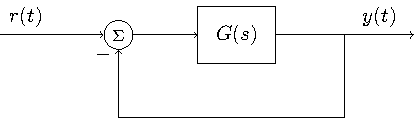
\includegraphics[width=.6\linewidth]{../../figures/block-simple-feedback}
\end{center}

Transfer function from \(r(t)\) to \(y(t)\):
\[ \frac{Y(s)}{R(s)} = \frac{G(s)}{ 1+ G(s)}\]

\pause
\alert{Mason's} gain formula: \(G_c(s) = \frac{Y(s)}{R(s)} = \frac{\sum_k T_k\Delta_k}{\Delta}\)

For simple systems with one loop only: \[G_c(s) = \frac{Y(s)}{R(s)} = \frac{\text{Forward path gain}}{1+\text{Loop gain}}\]
\end{frame}




\begin{frame}[label={sec:org5b4dfeb}]{Block diagram algebra}
\alert{Activity} Pair the block-diagram with the correct closed-loop transfer function!


\begin{longtable}{cccc}
\textcolor{red}{A} & \textcolor{red}{B} & \textcolor{red}{C} & \textcolor{red}{D}\\
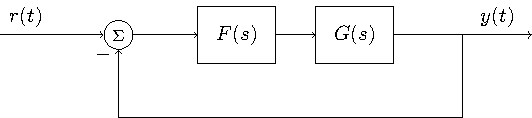
\includegraphics[width=3cm]{../../figures/block-simple-control-feedback} & 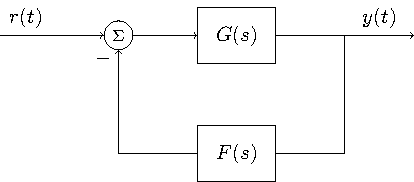
\includegraphics[width=3cm]{../../figures/block-simple-control-feedback2} & 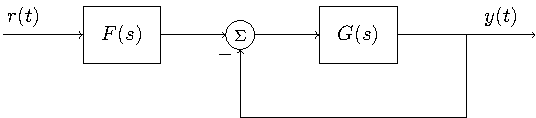
\includegraphics[width=3cm]{../../figures/block-simple-control-feedback3} & 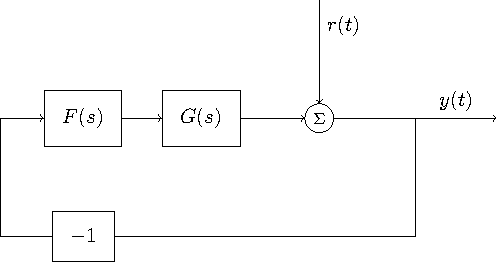
\includegraphics[width=3cm]{../../figures/block-simple-control-feedback4}\\
\end{longtable}


\begin{longtable}{cccc}
\textcolor{blue!80!black}{I} & \textcolor{blue!80!black}{II} & \textcolor{blue!80!black}{III} & \textcolor{blue!80!black}{IV}\\
\(\frac{Y(s)}{R(s)}=\frac{G(s)F(s)}{1 + G(s)}\) & \(\quad \frac{Y(s)}{R(s)}=\frac{G(s)}{1 + G(s)F(s)}\quad\) & \(\frac{Y(s)}{R(s)}=\frac{1}{1 + G(s)F(s)}\) & \(\frac{Y(s)}{R(s)}=\frac{G(s)F(s)}{1 + G(s)F(s)}\)\\
\end{longtable}
\end{frame}



\section{Proportional control of the DC motor}
\label{sec:orga100b65}

\begin{frame}[label={sec:org799eb1e}]{The DC motor}
\begin{columns}
\begin{column}{0.5\columnwidth}
\begin{center}
 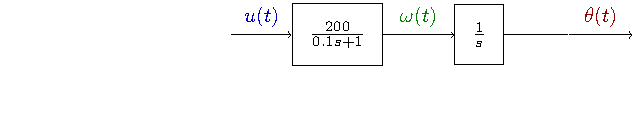
\includegraphics[width=1.0\linewidth]{../../figures/block-DC-feedback-white}
\end{center}
\end{column}
\begin{column}{0.5\columnwidth}
\begin{center}
 \def\ggain{200}
 \def\Tcnst{0.1}
 \begin{tikzpicture}
   \begin{axis}[
   width=7cm,
   height=6cm,
   grid = both,
   xlabel = {Time [s]},
   ylabel = {Ang vel [rad/s]},
   %xtick = {0, \tdelay, \tone, \two},
   %xticklabels = {0, $\theta$, $\theta+\frac{\tau}{3}$, $\theta + \tau$},
   %ytick = {0, \yone, \ytwo, \uampl, \yfinal},
   %yticklabels = {0, $0.283y_{f}$, $0.632y_f$, $u_f$, $y_f$},
   xmin = -0.2, xmax=2,
   minor y tick num=9,
   minor x tick num=9,
   every major grid/.style={red, opacity=0.5},
   ]
     \addplot [thick, green!50!black, no marks, domain=-0.2:2, samples=100] {(x>0)*\ggain*(1 - exp(-(x/\Tcnst)))}; 
  \end{axis}
 \end{tikzpicture}
\end{center}


\pause

\alert{Activity} What is the angle (approximately) rotated by the motor after 0.1s starting from still?
\end{column}
\end{columns}
\end{frame}
\begin{frame}[label={sec:orgfc31248}]{The normalized DC motor}
\begin{columns}
\begin{column}{0.5\columnwidth}
\begin{center}
 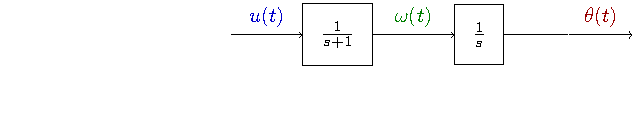
\includegraphics[width=1.0\linewidth]{../../figures/block-normalized-DC-feedback-white}
\end{center}
\end{column}

\begin{column}{0.5\columnwidth}
\begin{center}
 \def\ggain{1}
 \def\Tcnst{1}
 \begin{tikzpicture}
   \begin{axis}[
   width=7cm,
   height=6cm,
   grid = both,
   xlabel = {Time [$\tau$]},
   ylabel = {Ang vel [20 rad/$\tau$], angle [20 rad]},
   %xtick = {0, \tdelay, \tone, \two},
   %xticklabels = {0, $\theta$, $\theta+\frac{\tau}{3}$, $\theta + \tau$},
   %ytick = {0, \yone, \ytwo, \uampl, \yfinal},
   %yticklabels = {0, $0.283y_{f}$, $0.632y_f$, $u_f$, $y_f$},
   xmin = -2, xmax=20,
   minor y tick num=9,
   minor x tick num=9,
   every major grid/.style={red, opacity=0.5},
   ]
     \addplot [thick, green!50!black, no marks, domain=-2:20, samples=100] {(x>0)*\ggain*(1 - exp(-(x/\Tcnst)))};
     \addplot [thick, red!60!black, no marks, domain=-0.2:5, samples=100] {(x>0)*\ggain*(x + exp(-(x/\Tcnst)) -1)};
   \end{axis}
 \end{tikzpicture}
\end{center}

\pause
\alert{Activity} What is the settling time (approximately) for the velocity (in \(\tau\) and in seconds)?
\end{column}
\end{columns}
\end{frame}


\begin{frame}[label={sec:org21ba7f1}]{Proportional control of the normalized DC motor}
\begin{columns}
\begin{column}{0.5\columnwidth}
\begin{center}
 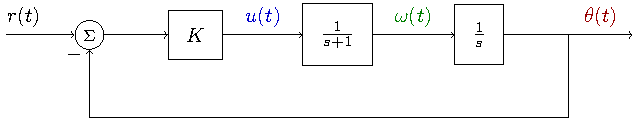
\includegraphics[width=1.0\linewidth]{../../figures/block-DC-feedback}
\end{center}

\pause
\end{column}
\begin{column}{0.5\columnwidth}
\begin{center}
 \def\ggain{1}
 \def\Tcnst{1}
 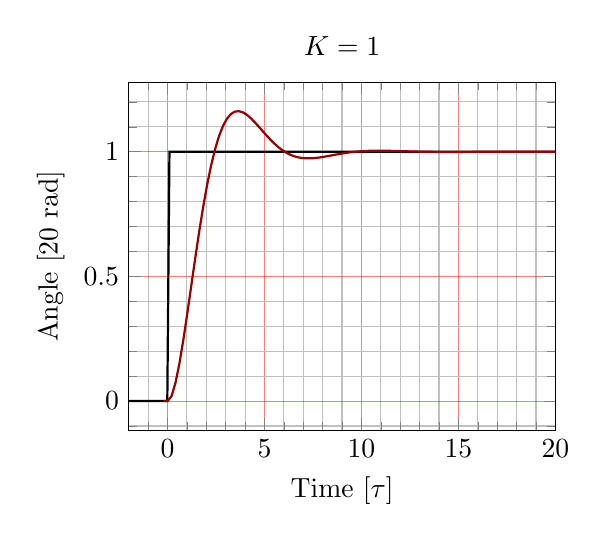
\begin{tikzpicture}
   \begin{axis}[
   width=7cm,
   height=6cm,
   grid = both,
   xlabel = {Time [$\tau$]},
   ylabel = {Angle [20 rad]},
   title = {$K=1$},
   %xtick = {0, \tdelay, \tone, \two},
   %xticklabels = {0, $\theta$, $\theta+\frac{\tau}{3}$, $\theta + \tau$},
   %ytick = {0, \yone, \ytwo, \uampl, \yfinal},
   %yticklabels = {0, $0.283y_{f}$, $0.632y_f$, $u_f$, $y_f$},
   xmin = -2, xmax=20,
   minor y tick num=4,
   minor x tick num=4,
   every major grid/.style={red, opacity=0.5},
   ]
     \addplot [thick, black, no marks, domain=-2:20, samples=200] {x>0};
     \addplot [thick, red!60!black, no marks, domain=-0.2:20, samples=100] {(x>0)*(1 - (exp(-x/2)* (sqrt(3)* cos(deg((sqrt(3)* x)/2)) + sin(deg((sqrt(3)* x)/2))))/sqrt(3))};
   \end{axis}
 \end{tikzpicture}
\end{center}


\pause
\alert{Activity} What is the overshoot (in percent) and rise time (in seconds)?
\end{column}
\end{columns}
\end{frame}



\begin{frame}[label={sec:orge679d4d}]{Proportional control of the normalized DC motor}
\begin{columns}
\begin{column}{0.5\columnwidth}
\begin{center}
 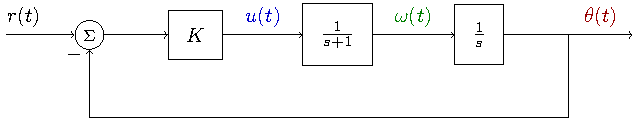
\includegraphics[width=1.0\linewidth]{../../figures/block-DC-feedback}
\end{center}
\end{column}

\begin{column}{0.5\columnwidth}
Closed-loop transfer function:
\[ G_c(s) = \frac{K}{s(s+1) + K}\]

Characteristic equation:
\[ s^2 + s + K = 0\]

\alert{Activity} Solve the characteristic equation!
\end{column}
\end{columns}
\end{frame}

\section{The root locus diagram}
\label{sec:org4970f26}

\begin{frame}[label={sec:orgd41484a}]{Root locus}
\begin{center}
 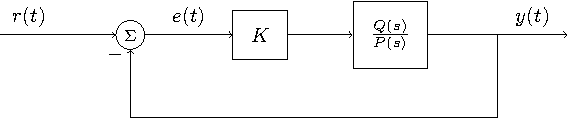
\includegraphics[width=1.0\linewidth]{../../figures/block-rlocus}
\end{center}

\alert{How do the closed-loop poles depend on \(K\)?}
\end{frame}

\begin{frame}[label={sec:org9835fe2}]{Root locus definition}
Let
\[\begin{cases} P(s)&=s^n+a_1s^{n-1}+\dots+a_n = (s-p_1)(s-p_2)\cdots(s-p_n)\\ 
Q(s)&=s^m+b_1s^{m-1}+\dots+b_m=(s-q_1)(s-q_2)\cdots(s-q_m) \end{cases},\ \ \ n\ge m \]
The root locus shows how the roots to the equation
\begin{equation}
\label{eq:P(s)+KQ(s)=0}
P(s)+K\cdot Q(s)=0,\ \ \ 0\le K<\infty
\end{equation}
depend on the parameter \(K\). The root locus consists of the set of all points in the complex plane that are roots to \eqref{eq:P(s)+KQ(s)=0} for some non-negative value of \(K\).
\end{frame}

\begin{frame}[label={sec:org39778df}]{Characteristics of the root locus}
The polynomial \(P(s)+KQ(s)=0\) above will always have \(n\) roots. Each gives a \emph{branch} in the root locus. Since the polynomials \(P(s)\) and \(Q(s)\) have real-valued coefficients, all roots are either real or complex-conjugated pairs. This means that the root locus is \emph{symmetric about the real axis.} Other characteristics
\begin{itemize}
\item Start points - marked by crosses
\item End points - marked  by circles
\item Asymptotes
\item Pieces of the real axis
\end{itemize}
\end{frame}

\begin{frame}[label={sec:org30616d2}]{Start- and end points}
\begin{description}
\item[{Start points}] These are the \(n\) roots of \(P(s) + KQ(s)\) for \(K=0\), i.e. the roots of \(P(s)\). These are the open-loop poles, and are marked with crosses '\(\times\)'
\item[{End points}] These are the \(m\) (finite) roots of \(P(s)+KQ(s)\) when \(K\to\infty\), and are hence the roots of \(Q(s)\). The end points are marked with circles '\(\circ\)'
\end{description}
\end{frame}

\begin{frame}[label={sec:orgeba0533}]{The real axis}
Those parts of the real axis that have an \alert{odd number} of real-valued start- or end points to the right (including multiplicity) belong to the root locus. 
\end{frame}


\begin{frame}[label={sec:org4bf6958}]{Asymptotes, directions}
The directions of the asymptotes are given by the expression
\[ \theta_k = \arg s = \frac{(2k+1)\pi}{n-m}, \; k \in \mathbb{Z} \]
Example: 6 start points and 3 end points gives \(n-m = 6-3 = 3\) and the directions

\begin{columns}
\begin{column}{0.35\columnwidth}
\[ \theta = \begin{cases} \frac{\pi}{3}, & k=0\\ \pi, & k=1\\ -\frac{\pi}{3}, & k=-1 \end{cases}. \]
\end{column}

\begin{column}{0.65\columnwidth}
\begin{center}
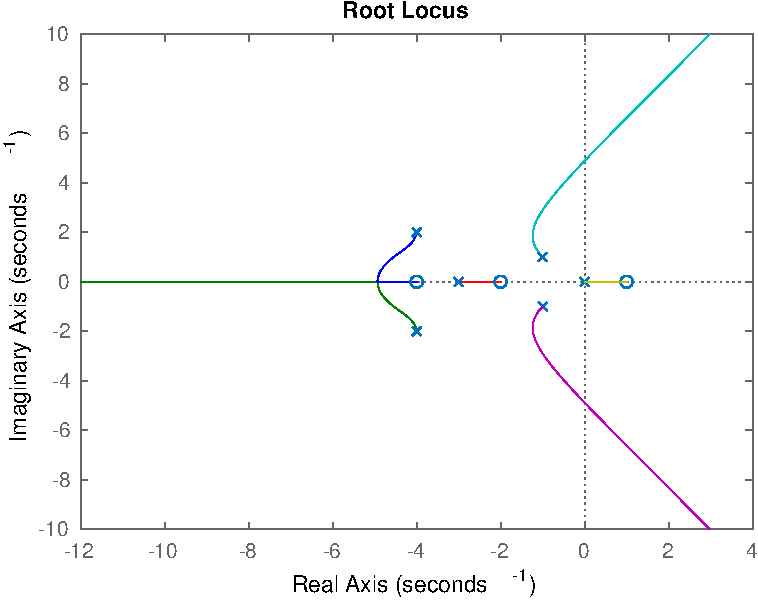
\includegraphics[width=0.8\linewidth]{root-locus-ex-3asymptotes-crop}
\end{center}
\end{column}
\end{columns}
\end{frame}

\begin{frame}[label={sec:org0b3a832}]{Asymptotes, intersection with the real axis}
\begin{columns}
\begin{column}{0.4\columnwidth}
\[ ip = \frac{ \sum_{i=1}^n p_i - \sum_{i=1}^m q_i}{n-m}, \]
where \(\{p_i\}\) are the starting points (open-loop poles) and \(\{q_i\}\) are the end points (open-loop zeros). 
\end{column}

\begin{column}{0.6\columnwidth}
\pgfmathsetmacro{\impart}{sqrt(3)/2}
 \begin{center}
\small
   \begin{tikzpicture}[scale=1.4, block/.style={draw, minimum width=12mm, minimum height=8mm},]
   \draw[->] (-4, 0) -- node[right, pos=1] {Re} (0.5, 0);
   \draw[->] (0, -1.3) -- node[right, pos=0.96] {Im} (0, 1.3);
   \draw (-1, 0) -- ++(0,-0.2) node[below] {-1};
   \draw (-2, 0) -- ++(0,-0.2) node[below] {-2};
   \draw (-3, 0) -- ++(0,-0.2) node[below] {-3};
   \node[red, ] at (0,0) {\large $\times$};
   \node[red] at (-1, 0) {\large $\times$};
   \node[red] at (-3, 0) {\large $\times$};
   \node[green!80!black,] at (-2, 0) {\large $\circ$};
   %\node[green!80!black] at (-0.5, 0) {\large $\circ$};

   \end{tikzpicture}

 \end{center}
\end{column}
\end{columns}
\end{frame}


\section{Examples}
\label{sec:org9e8f3dd}

\begin{frame}[label={sec:org3b1b3e2}]{Examples}
\end{frame}

\begin{frame}[label={sec:org8ebc182}]{Motor driving an elastic shaft}
 \small
 \begin{center}
   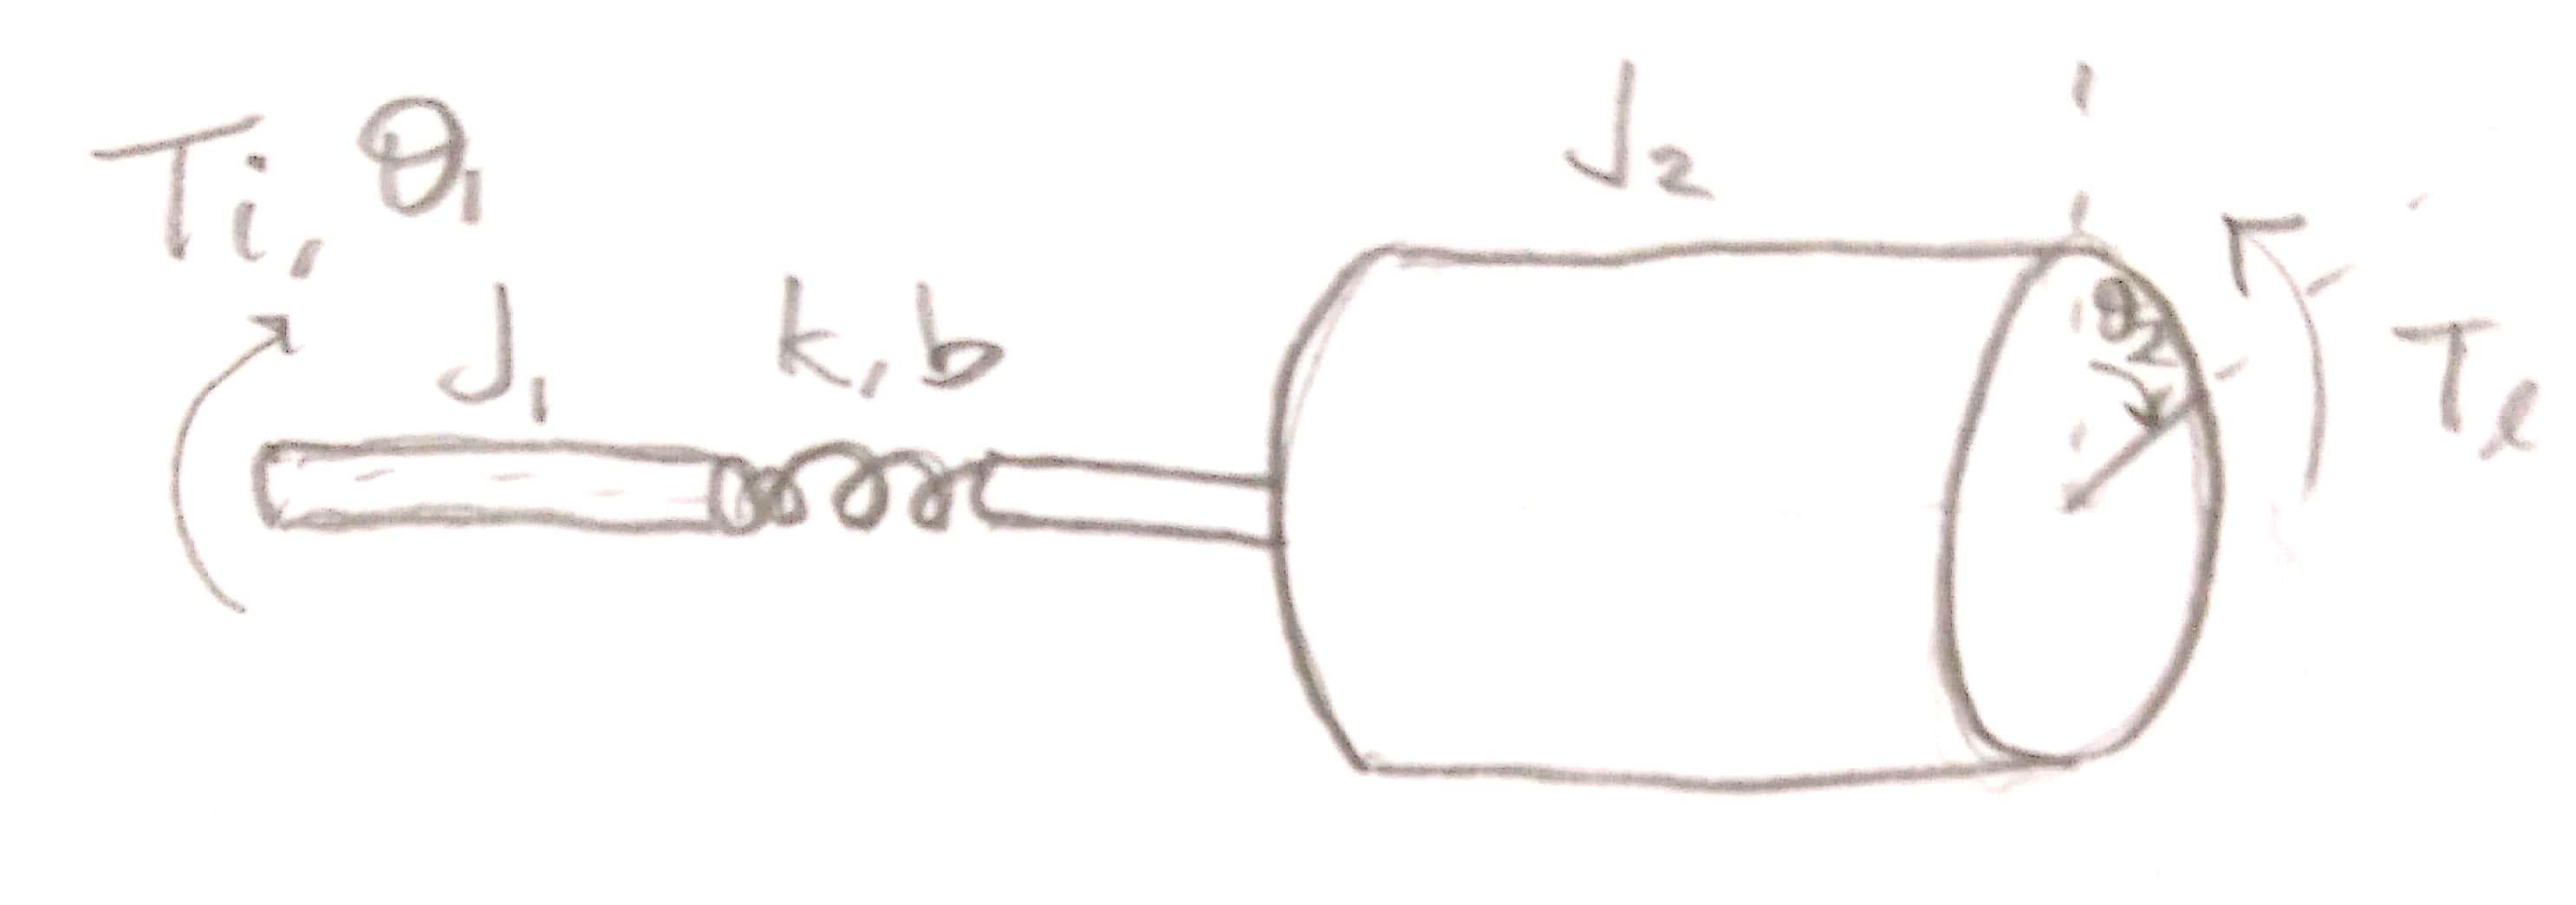
\includegraphics[width=0.4\linewidth]{../../figures/elastic-shaft.jpg}

   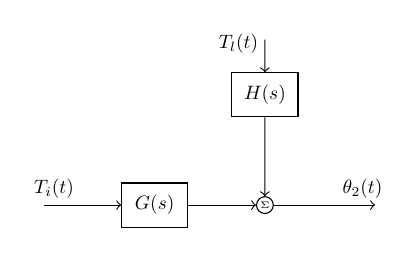
\begin{tikzpicture}[scale=0.7, transform shape, block/.style={draw, minimum width=12mm, minimum height=8mm},]
     \node[block] (plant) {$G(s)$};
     \node[circle, draw, inner sep=1pt, right of=plant, node distance=2cm] (sum) {\tiny $\Sigma$};
     \node[block, above of=sum, node distance=2cm] (load) {$H(s)$};
     \draw[->] (plant) ++ (-2cm, 0) -- node[very near start, above] {$T_i(t)$} (plant);
     \draw[->] (load) ++ (0,1cm) -- node[very near start, left] {$T_l(t)$} (load);
     \draw[->] (plant) -- (sum);
     \draw[->] (load) -- (sum);
     \draw[->] (sum) -- node[very near end, above] {$\theta_2(t)$} ++(2cm, 0);
   \end{tikzpicture}

   \end{center}

\begin{align*}
\Theta_2(s) &= \underbrace{\frac{k + bs}{s^2(J_1J_2s^2 + bs + k)}}_{G(s)}T_i(s) \underbrace{- \frac{J_1s^2 + bs + k}{s^2(J_1J_2s^2 + bs + k)}}_{H(s)}T_l(s)
   \end{align*}
\end{frame}

\begin{frame}[label={sec:orgd640ec7}]{Motor driving an elastic shaft}
\begin{columns}
\begin{column}{0.4\columnwidth}
PD-control

\begin{center}
  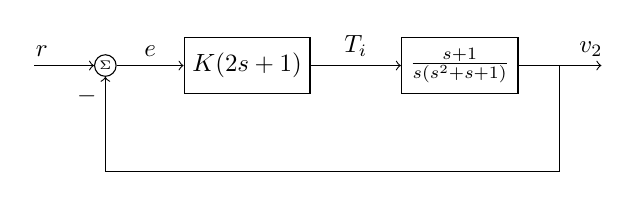
\begin{tikzpicture}[scale=0.9, transform shape, block/.style={draw, minimum width=12mm, minimum height=8mm},]
    \node[block] (plant) {$\frac{s+1}{s(s^2 + s + 1)}$};
    \node[block, left of=plant, node distance=3cm] (pd) {$K(2s + 1)$};
    \node[circle, draw, inner sep=1pt, left of=pd, node distance=2cm] (sum) {\tiny $\Sigma$};
    \node[coordinate, left of=sum,] (input) {};
    \draw[->] (input) -- node[very near start, above] {$r$} (sum);
    \draw[->] (sum) -- node[ above] {$e$} (pd);
    \draw[->] (pd) -- node[above] {$T_i$} (plant);
    \draw[->] (plant) -- node[coordinate] (meas) {}
            node[very near end, above] {$v_2$} ++(2cm, 0);
    \draw[->] (meas) -- ++(0, -15mm) -| node[left, pos=0.9] {$-$} (sum);
  \end{tikzpicture}
\end{center}
\end{column}
\begin{column}{0.6\columnwidth}
\pgfmathsetmacro{\impart}{sqrt(3)/2}
 \begin{center}
\small
   \begin{tikzpicture}[scale=1.4, block/.style={draw, minimum width=12mm, minimum height=8mm},]
   \draw[->] (-2, 0) -- node[right, pos=1] {Re} (0.5, 0);
   \draw[->] (0, -1.3) -- node[right, pos=0.96] {Im} (0, 1.3);
   \draw (0,\impart) -- ++(0.2, 0) node[right] {$i\frac{\sqrt{3}}{2}$};
   \draw (0,-\impart) -- ++(0.2, 0) node[right] {$-i\frac{\sqrt{3}}{2}$};
   \draw (-0.5, 0) -- ++(0,-0.2) node[below] {-0.5};
   \draw (-1, 0) -- ++(0,-0.2) node[below] {-1};
   %\node[red, ] at (0,0) {\large $\times$};
   %\node[red] at (-0.5, \impart) {\large $\times$};
   %\node[red] at (-0.5, -\impart) {\large $\times$};
   %\node[green!80!black,] at (-1, 0) {\large $\circ$};
   %\node[green!80!black] at (-0.5, 0) {\large $\circ$};

   \end{tikzpicture}

 \end{center}

\alert{Activity} Indicate the start- and end points.
\end{column}
\end{columns}
\end{frame}



\begin{frame}[label={sec:org51c1623}]{Motor driving an elastic shaft}
\begin{center}
  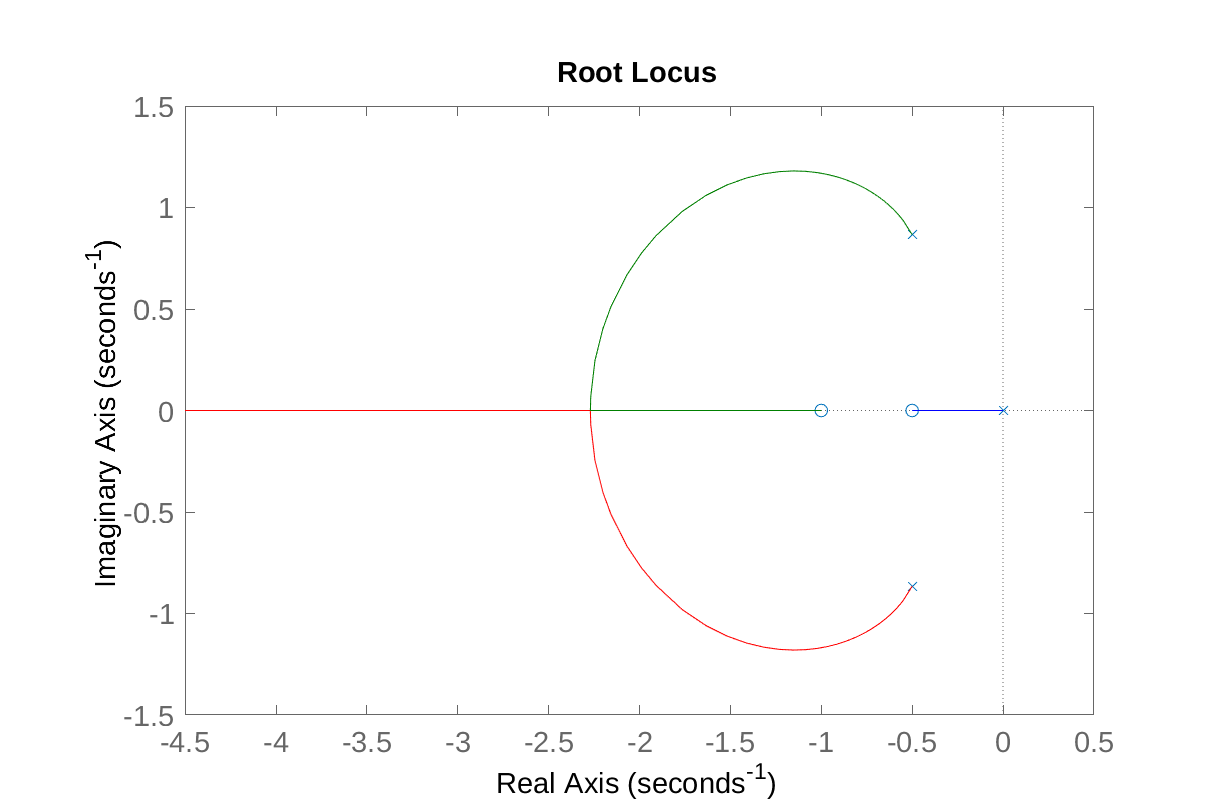
\includegraphics[width=.7\linewidth]{../../figures/shaft-rlocus}
\end{center}
\end{frame}

\begin{frame}[label={sec:orgb89c6ed}]{Harmonic oscillator}
\begin{columns}
\begin{column}{0.4\columnwidth}
P-control

\begin{center}
  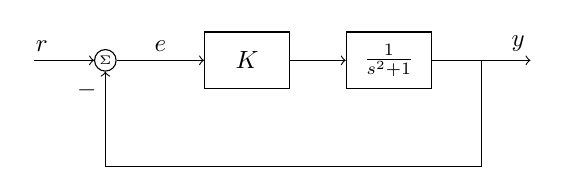
\begin{tikzpicture}[scale=0.9, transform shape, block/.style={draw, minimum width=12mm, minimum height=8mm},]
    \node[block] (plant) {$\frac{1}{s^2 + 1}$};
    \node[block, left of=plant, node distance=2cm] (pd) {$K$};
    \node[circle, draw, inner sep=1pt, left of=pd, node distance=2cm] (sum) {\tiny $\Sigma$};
    \node[coordinate, left of=sum,] (input) {};
    \draw[->] (input) -- node[very near start, above] {$r$} (sum);
    \draw[->] (sum) -- node[ above] {$e$} (pd);
    \draw[->] (pd) -- node[above] {} (plant);
    \draw[->] (plant) -- node[coordinate] (meas) {}
            node[very near end, above] {$y$} ++(2cm, 0);
    \draw[->] (meas) -- ++(0, -15mm) -| node[left, pos=0.9] {$-$} (sum);
  \end{tikzpicture}
\end{center}
\end{column}
\begin{column}{0.6\columnwidth}
\pgfmathsetmacro{\impart}{sqrt(3)/2}
 \begin{center}
\small
   \begin{tikzpicture}[scale=1.4, block/.style={draw, minimum width=12mm, minimum height=8mm},]
   \draw[->] (-3, 0) -- node[right, pos=1.02] {Re} (0.5, 0);
   \draw[->] (0, -1.3) -- node[right, pos=0.96] {Im} (0, 1.3);
   \draw (0,\impart) -- ++(0.2, 0) node[right] {$i$};
   \draw (0,-\impart) -- ++(0.2, 0) node[right] {$-i$};
   %\draw (-0.5, 0) -- ++(0,-0.2) node[below] {-0.5};
   \draw (-1, 0) -- ++(0,-0.2) node[below] {-1};
   %%\node[red, ] at (0,0) {\large $\times$};
   %\node[red] at (-0.5, \impart) {\large $\times$};
   %\node[red] at (-0.5, -\impart) {\large $\times$};
   %\node[green!80!black,] at (-1, 0) {\large $\circ$};
   %\node[green!80!black] at (-0.5, 0) {\large $\circ$};

   \end{tikzpicture}

 \end{center}

\alert{Activity} Indicate the start- and end points, and the asymptotes.
\end{column}
\end{columns}
\end{frame}



\begin{frame}[label={sec:orgb98a32b}]{Harmonic oscillator}
\begin{columns}
\begin{column}{0.4\columnwidth}
Lead-compensator

\begin{center}
  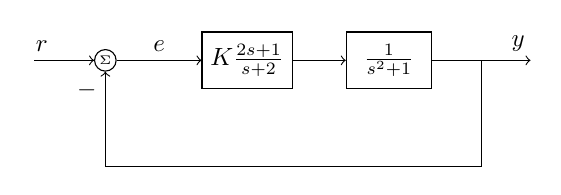
\begin{tikzpicture}[scale=0.9, transform shape, block/.style={draw, minimum width=12mm, minimum height=8mm},]
    \node[block] (plant) {$\frac{1}{s^2 + 1}$};
    \node[block, left of=plant, node distance=2cm] (pd) {$K\frac{2s + 1}{s+2}$};
    \node[circle, draw, inner sep=1pt, left of=pd, node distance=2cm] (sum) {\tiny $\Sigma$};
    \node[coordinate, left of=sum,] (input) {};
    \draw[->] (input) -- node[very near start, above] {$r$} (sum);
    \draw[->] (sum) -- node[ above] {$e$} (pd);
    \draw[->] (pd) -- node[above] {} (plant);
    \draw[->] (plant) -- node[coordinate] (meas) {}
            node[very near end, above] {$y$} ++(2cm, 0);
    \draw[->] (meas) -- ++(0, -15mm) -| node[left, pos=0.9] {$-$} (sum);
  \end{tikzpicture}
\end{center}
\end{column}
\begin{column}{0.6\columnwidth}
\pgfmathsetmacro{\impart}{sqrt(3)/2}
 \begin{center}
\small
   \begin{tikzpicture}[scale=1.4, block/.style={draw, minimum width=12mm, minimum height=8mm},]
   \draw[->] (-3, 0) -- node[right, pos=1.02] {Re} (0.5, 0);
   \draw[->] (0, -1.3) -- node[right, pos=0.96] {Im} (0, 1.3);
   \draw (0,\impart) -- ++(0.2, 0) node[right] {$i$};
   \draw (0,-\impart) -- ++(0.2, 0) node[right] {$-i$};
   \draw (-0.5, 0) -- ++(0,-0.2) node[below] {-0.5};
   \draw (-2, 0) -- ++(0,-0.2) node[below] {-2};
   %%\node[red, ] at (0,0) {\large $\times$};
   %\node[red] at (-0.5, \impart) {\large $\times$};
   %\node[red] at (-0.5, -\impart) {\large $\times$};
   %\node[green!80!black,] at (-1, 0) {\large $\circ$};
   %\node[green!80!black] at (-0.5, 0) {\large $\circ$};

   \end{tikzpicture}

 \end{center}

\alert{Activity} Indicate the start- and end points, and the asymptotes.
\end{column}
\end{columns}
\end{frame}



\begin{frame}[label={sec:org73b4861}]{Pair the root locus plots with the correct transfer function}
\begin{columns}
\begin{column}{0.3\columnwidth}
\begin{align*}
G_1(s) &= K\frac{s+2}{s(s+4)}\\ G_2(s) &= K\frac{s+2}{s(s+4)(s+8)}\\
G_3(s) &= K\frac{s+2}{s^2(s+4)}\\ G_4(s) &= K \frac{1}{s^2(s+4)}.
\end{align*}

\begin{center}
 \includegraphics[width=1.0\linewidth]{../../figures/}
\end{center}
\end{column}
\begin{column}{0.7\columnwidth}
\begin{center}
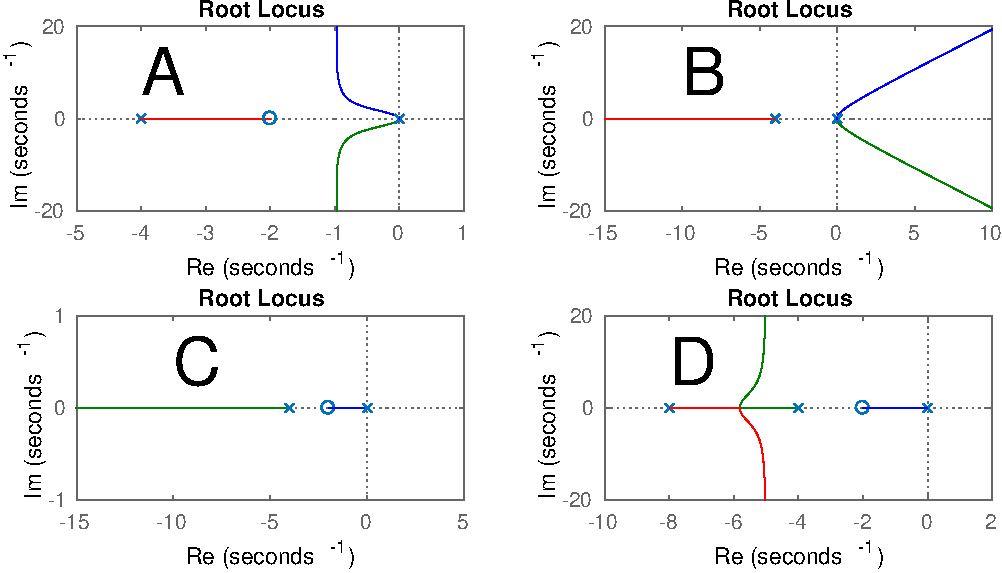
\includegraphics[width=1.0\linewidth]{../../figures/rlocus_2x2-crop}
\end{center}
\end{column}
\end{columns}
\end{frame}
\end{document}